\documentclass[titlepage]{article}
\usepackage{mathptmx}
\usepackage{fancyhdr}
\usepackage{float}
\usepackage{setspace}
\usepackage{graphicx, subfigure}
\usepackage[right=1.25in,left=1.25in]{geometry}
\lhead{Cosc 5P01 - Presentation Proposal}
\rhead{Justin Maltese (\#4738274)}
\begin{document}
\doublespacing
\author{Justin Maltese}
\title{CICC Framework User Manual}
\maketitle
\def\code#1{\texttt{#1}}


\tableofcontents

\section{Overview}
\subsection{Motivation}

The Computational Intelligence for Covering Codes (CICC) framework is a tool for developers to implement custom computational intelligence algorithms for the purpose of finding minimal covering codes. Currently, no frameworks exist for this purpose, thus the primary motivation for the CICC framework is to fill this gap. At its core, the CICC framework serves to compare all types of computational intelligence algorithms on minimal covering problems, running comparisons as quick as possible and saving results in an easy-to-read format. Algorithm implementation aims to be simple, representing a plug-and-play style framework. It is our hope that developers can utilize the CICC framework to avoid writing boilerplate code, instead focussing on implementing creative new computational intelligence algorithms.
\subsection{Feature Summary}

The CICC framework provides a variety of different features, which include the following:

\begin{itemize}
\item Sleek graphical interface for users to select algorithms and minimal covering code problems for comparison purposes in a step-by-step fashion
\item Fast, easy comparison of algorithms on the minimal covering code problem
\item Live updates of algorithm performance
\item Automatic saving of best-ever-found minimal covering codes. Upon finding a new best-ever code for a problem, the code is written out as a .code file to the \textit{Codes} folder.
\item Ability to easily implement new CI algorithms along with respective parameter sets in a plug-and-play fashion
\item Developers can setup algorithm comparisons directly in code rather than using a graphical interface
\item Ability to automatically write comparison results into nicely-formatted LaTeX tables
\end{itemize}

\section{Installation}

Upon downloading the executable version of the CICC framework, the package should contain the files shown below:

\begin{figure}[H]
\centering
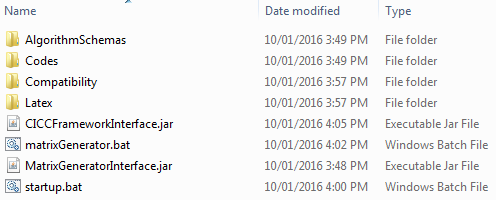
\includegraphics[width=100mm]{Images/Installation.png}
\end{figure}

To run the graphical user interface, simply execute the \textbf{startup.bat} file. Note that if either the CICCFrameworkInterface.jar file or the AlgorithmSchemas folder is missing, the program will not execute. Please ensure that both of these items are present.

\section{Architecture}

\subsection{Basic Components}

The basic components of the CICCFramework are \textbf{solutions}, \textbf{algorithms} and \textbf{problems}. Within the CICC framework, all algorithms evolve small ``seeds" which are fed into a greedy algorithm to produce full covering codes. This has the advantage of keeping candidate solution representation small and compact, minimizing epistasis. Each solution represents a ``seed", possessing a set of decision variables which are analogous to codewords present in the seed. All codewords are represented as integers, stored in memory as the corresponding base-2 representation.

Algorithms within the CICC framework extend the \code{Algorithm} class. Each algorithm typically possesses a set of solutions, formally referred to as a \code{SolutionSet}, which are modified in some way during the execution of the algorithm. All operations performed by the algorithm should be placed into a method with the signature \code{public Solution execute()}. This method should return the overall best solution found by the algorithm during execution. Algorithms can print an output message using the \code{printLine(String)} method.

Problems represent minimal covering code problems, formally referred to as $K_q(n,r)$. Thus, a problem requires a value for $q$, $n$ and $r$. Additionally, since all algorithms within the CICC framework are \textit{greedy closure algorithms}, each problem requires a $seed\_size$ integer parameter which corresponds to the size of the seeds (candidate solutions) evolved by each algorithm.

\subsection{XML Schemas}

When defining a new algorithm in the CICC framework, an XML file must be provided for the algorithm  in the $AlgorithmSchemas$ folder which defines its properties and parameters. The root element should be \code{algorithm}, possessing the following attributes:

\begin{itemize}
\item \textbf{id} - abbreviation which uniquely identifies the algorithm
\item \textbf{name} - full name of the algorithm
\item \textbf{driverClass} - full path (including package prefixes) to the algorithm class containing the \code{execute()} method
\end{itemize}

Nested within the \code{algorithm} element should be the \code{parameterSet} element. Each parameter of the algorithm should be given as a \code{parameter} child element within the \code{parameterSet} element. Parameters should possess the following attributes:

\begin{itemize}
\item \textbf{id} - string which uniquely identifies the parameter
\item \textbf{label} - label of the parameter, displayed to the user via the GUI
\item \textbf{type} - type of the parameter. Possible values are {Integer, Double, Float, Long, Boolean}
\item \textbf{defaultValue} (optional) - default value of the parameter
\end{itemize}

A sample XML schema for a discrete particle swarm optimization algorithm is provided below.

\begin{figure}[H]
\centering
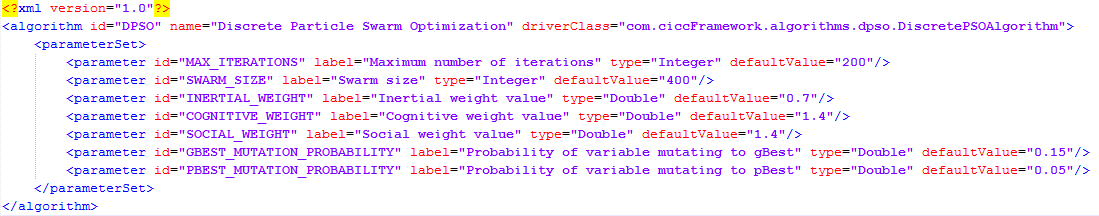
\includegraphics[width=180mm]{Images/SchemaExample.png}
\end{figure}


\subsection{Fitness Evaluation}

To ensure a plug-and-play style, fitness evaluation of solutions is extremely easy to perform when implementing an algorithm. Since each algorithm should possess a \code{SolutionSet} (see Section 3.1) containing the candidate solutions of the algorithm, the \code{doEvaluation()} method of the solution set can be called to perform fitness evaluation of all solutions in the set. Note that fitness evaluations are distributed across all available cores to minimize the amount of time taken. Upon completing the \code{doEvaluation} method, the \code{fitness} property of each solution will be updated with its corresponding fitness value. Note that solutions which possess invalid codewords (boundary violations) are given a fitness of \code{Integer.MAX\_VALUE}.

\subsection{Codeword Compatibility}

Computing the compatibility between codewords is an important task in the CICC framework. Since codewords are stored in memory as binary representations, problems possessing $q = 2$ utilize bit operations to swiftly calculate codeword compatibility. When $q > 3$, the integer representation of each word is converted into base $q$ when computing distance. In this case, bit operations cannot be used and thus compatibility calculation is much slower. Consequently word compatibility is not computed at runtime, rather it is precomputed and accessed in $O(1)$ time via a matrix of bits. Such a matrix is deemed a ``compatibility matrix", defined as follows: Let $H_D(x,y)$ represent the Hamming distance between integer words x and y. If the bit at index $i,j$ = 1, $H_D(i,j) \leq r$, therefore $i$ covers $j$ and vice-versa. If the index is 0, then neither $i$ or $j$ cover each other and thus are incompatible.

\subsubsection{Generating Compatibility Matrices}

Problems with $q>3$ require pre-computed compatibility matrices, stored in .matrix files within the $Compatibility$ folder. Using this strategy, large values of $n$ and $q$ can be tackled for as many runs as needed, since the matrix only needs to be loaded into memory once for a given problem. The \textbf{matrixGeneration.bat} file can be executed to bring up an interface which allows compatibility matrices to be generated up to a specified problem parameter set. To save memory, redundant information of compatibility matrices is removed. This includes the upper triangular portion of the matrix (since the matrix is mirrored) and the diagonal of the matrix (since $H_D(i,i) = 0$ trivially). An example compatibility matrix for the $K_3(3,2)$ problem is shown in Figure 1.

\begin{figure}[H]
\centering
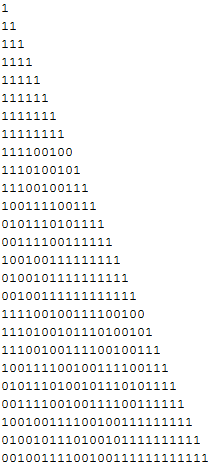
\includegraphics[width=40mm]{Images/CompatibilityMatrix.png}
\caption{Compatibility matrix for the $K_3(3,2)$ is displayed.}
\end{figure}

\section{Experimentation}

\subsection{Graphical User Interface}

Using the graphical user interface to perform experimentation is straightforward:

\textbf{Step 1:} Startup the graphical user interface via \textbf{startup.bat}

\begin{figure}[H]
\centering
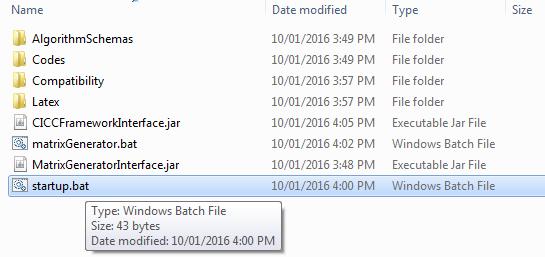
\includegraphics[width=90mm]{Images/guiSteps/step1.png}
\end{figure}

\textbf{Step 2:} Select an algorithm for comparison and click the ``Add" button

\begin{figure}[H]
\centering
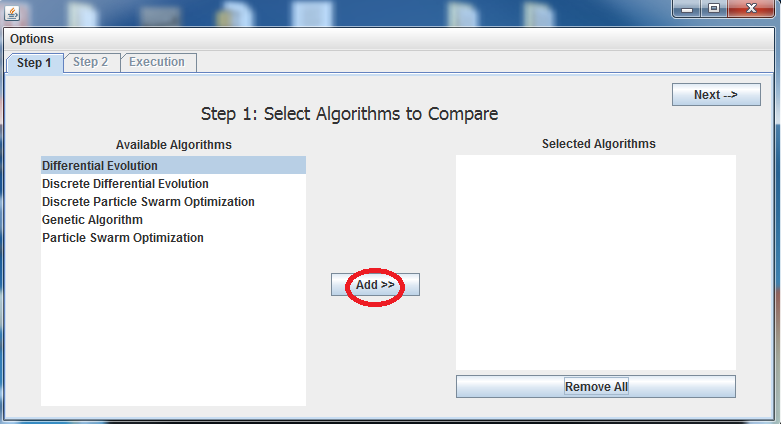
\includegraphics[width=150mm]{Images/guiSteps/step2.png}
\end{figure}

\textbf{Step 3:} Select a set of parameters for the added algorithm and click the ``Save" button

\begin{figure}[H]
\centering
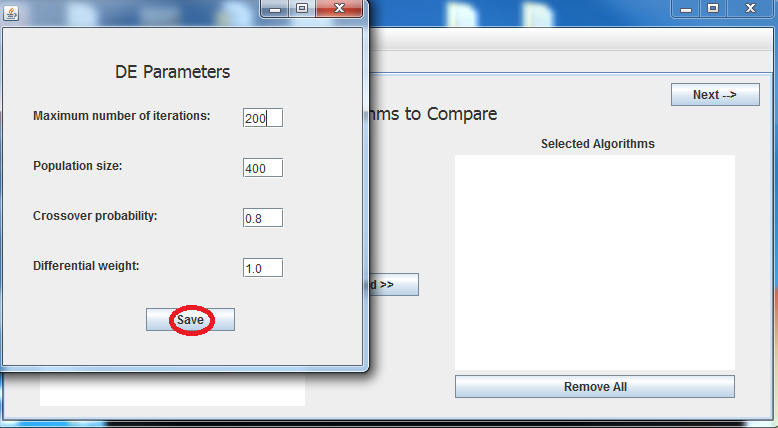
\includegraphics[width=160mm]{Images/guiSteps/step3.png}
\end{figure}

\textbf{Step 4:} When all desired algorithms have been added, click the ``Next" button to continue

\begin{figure}[H]
\centering
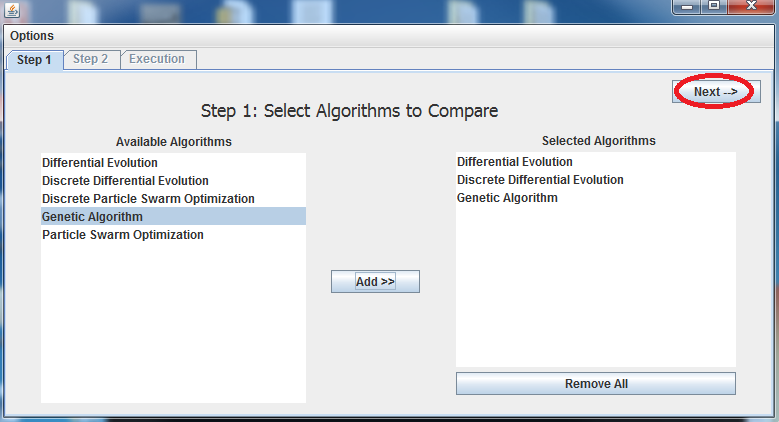
\includegraphics[width=150mm]{Images/guiSteps/step4.png}
\end{figure}

\textbf{Step 5:} Select a set of parameters for a desired problem and click the ``Add" button

\begin{figure}[H]
\centering
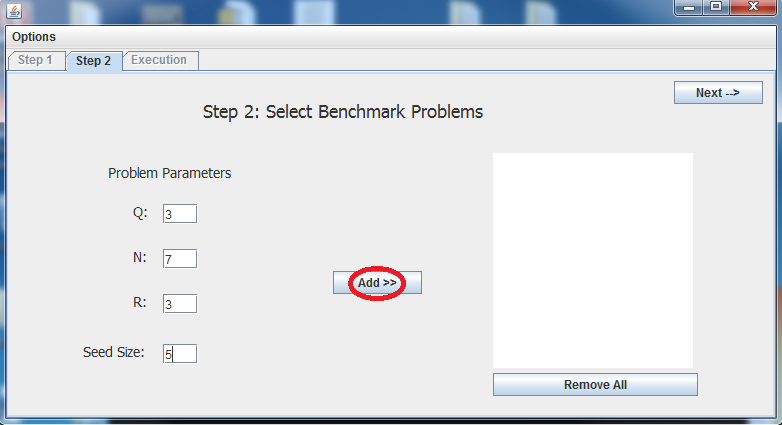
\includegraphics[width=160mm]{Images/guiSteps/step5.png}
\end{figure}

\textbf{Step 6:} When all desired problems have been added, click the ``Next" button to continue

\begin{figure}[H]
\centering
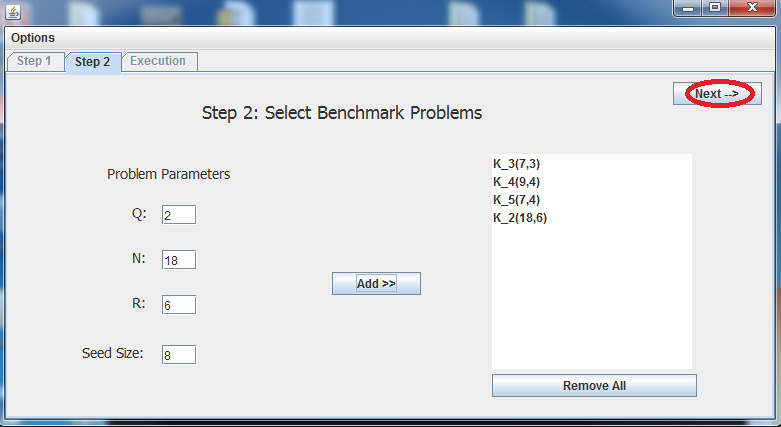
\includegraphics[width=150mm]{Images/guiSteps/step6.png}
\end{figure}

\textbf{Step 7:} Allow the algorithms to execute on each problem in the execution pane

\begin{figure}[H]
\centering
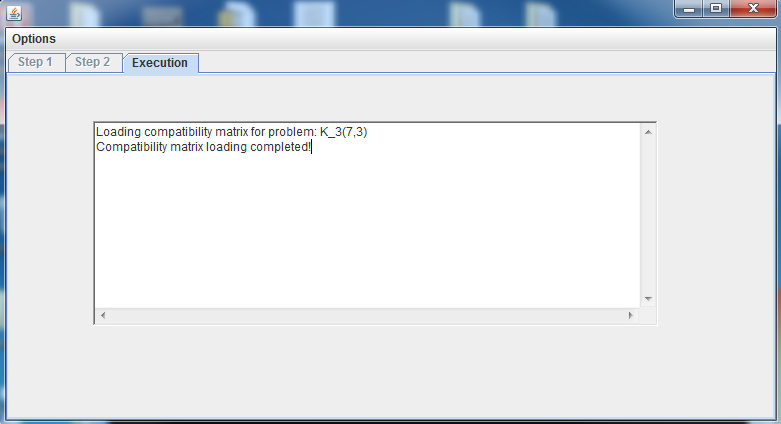
\includegraphics[width=160mm]{Images/guiSteps/step7.png}
\end{figure}

\textbf{Step 8:} When all experiments have completed, results formatted as LaTeX tables can be viewed via \textit{Latex/output.tex}

\begin{figure}[H]
\centering
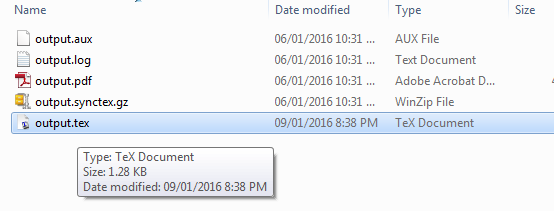
\includegraphics[width=160mm]{Images/guiSteps/step8.png}
\end{figure}

\clearpage

\subsection{ExecutionHandler}

Experiments can also be run manually in new .java files using the \code{ExecutionHandler} class. The following sequence of steps are required for this purpose:

\begin{enumerate}
\item Create a new \code{ExecutionHandler} object
\item Load a hashmap of all available algorithm schemas using \code{XMLSchemaLoader.loadAlgorithmSchemas()}
\item Retrieve the desired algorithm schemas from the schema map by ID
\item Create \code{ParameterSet} objects for each algorithm and add the desired parameters to each
\item Add algorithm instances to the \code{ExecutionHandler} using the \code{attachAlgorithmInstance} method, passing in an algorithm schema and the corresponding parameter set
\item Create problems as \code{CoveringProblem} objects with the desired parameters
\item Add problem instances to the \code{ExecutionHandler} using the \code{attachProblemInstance} method, passing in each problem
\item Customize the \code{ExecutionHandler} as desired, setting items such as the output path (\code{setOutputPath)} and number of runs (\code{setNumRuns})
\item Execute the \code{ExecutionHandler} by calling the \code{run()} method
\end{enumerate}

A comprehensive example of how to use the \code{ExecutionHandler} can be found on the following page.


\begin{figure}[H]
\centering
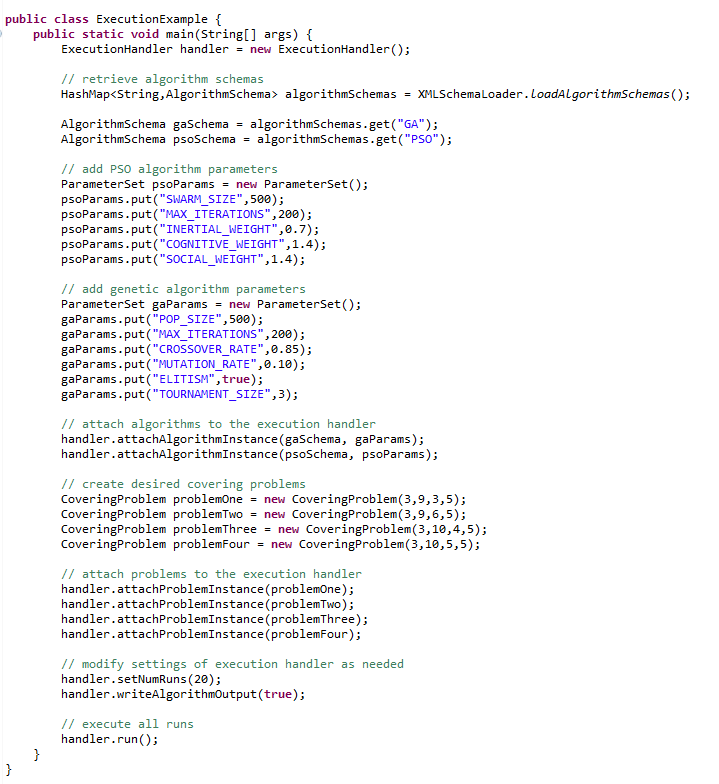
\includegraphics[width=190mm]{Images/ExecutionHandlerExample.png}
\end{figure}

\section{FAQ}

\begin{enumerate}
\item \textbf{Q: I am running out of memory when attempting to load/generate large compatibility matrices!} \\
\textbf{A:} Allocate more heap space by running java with arguments -Xmx \textit{\textless desired heap size\textgreater}

\item \textbf{Q: A runtime error is occurring stating that the compatibility matrix file is missing for the covering problem I'm trying to run?} \\
\textbf{A:} This error occurs when the compatibility matrix file has not been generated (or has been misplaced). The compatibility matrix can be generated using the matrix generator interface.

\item \textbf{Q: When loading algorithm schemas, the program throws an exception?} \\
\textbf{A:} This error occurs when their is a formatting problem within the XML schema files. Ensure that the file is in the correct format, detailed in Section 3.2.

\item \textbf{Q: When loading my desired algorithm schema, the loaded schema is incorrect!} \\
\textbf{A:} Ensure that the algorithm schema has an id attribute which is unique.

\item \textbf{Q: When writing results out in LaTeX format, the program is unable to write the file.} \\
\textbf{A:} Ensure that the chosen output path has full write permissions.

\item \textbf{Q: I want to use this framework to find optimal codes as well!} \\
\textbf{A:} Currently, the framework only supports covering codes. However, it is possible that in a future release optimal codes will be supported as well. Especially since the modifications required to accomodate optimal code problems are trivial.

\item \textbf{Q: Is there any way to turn off the automatic .code file saving for newly found bests?} \\
\textbf{A:} Currently, there is no way to turn off the automatic saving. It is a bad idea to do so, since .code files can be checked for errors to ensure that the program is not erroneously finding invalid minimal covering code bounds. This ensures the integrity of research which stems from experiments performed using the CICC framework.
\end{enumerate}



\end{document}